\label{sec:appendix}

%%%%%%%%%%%%%%%%%%%%%%%%%%%%%%%%%%%%%%%%%%%%%%%%%%%%%%%%%%%%%%%%%%
% Hyperparameters
%%%%%%%%%%%%%%%%%%%%%%%%%%%%%%%%%%%%%%%%%%%%%%%%%%%%%%%%%%%%%%%%%%
\begin{table*}[t]
\tiny
\centering
\caption{Detailed hyperparameters for depth diffusion models used for experiments in TABLE \ref{tab:depth_diffusion_ablation}}
\label{tab:experiment_model_description_depth_diffusion}
\begin{tabular}{ l || r r r r r r r r r r }
\textbf{Run} & \textbf{dd1} & \textbf{dd2} & \textbf{dd3} & \textbf{dd4} & \textbf{dd5} & \textbf{dd6} & \textbf{dd7} & \textbf{dd8} & \textbf{dd9} & \textbf{dd10} \\ 
\hline
\hline
 Model & UNet & UNet3+ & UNet3+ & UNet3+ & UNet3+ & UNet & UNet & UNet3+ & UNet3+ & UNet3+\\
 Diffusion Steps & 600 & 600 & 600 & 600 & 600 & 600 & 600 & 600 & 600 & 600\\
 Condition Input & RGB & RGB & RGB & RGB & RGB & RGB & RGB & RGB & RGB & RGB \\
 Noise Schedule & cosine & cosine & cosine & cosine & cosine & cosine & cosine & cosine & cosine & cosine \\
 Model Size & 41M & 42M & 42M & 42M & 42M & 41M & 41M & 42M & 55M & 55M \\
 Base Dim & 64 & 64 & 64 & 64 & 64 & 64 & 64 & 64 & 64 & 64 \\
 Base Dim Mult. & 1/2/4/8 & 1/2/4/8 & 1/2/4/8 & 1/2/4/8 & 1/2/4/8 & 1/2/4/8 & 1/2/4/8 & 1/2/4/8 & 1/2/4/8 & 1/2/4/8 \\
 \# Blocks & 1/1/1/1 & 1/1/1/1 & 1/1/1/1 & 1/1/1/1 & 1/1/1/1 & 1/1/1/1 & 1/1/1/1 & 1/1/1/1 & 1/1/1/1 & 1/1/1/1 \\
 \# ResNet Blocks & 2/2/2/2 & 2/2/2/2 & 2/2/2/2 & 2/2/2/2 & 2/2/2/2 & 2/2/2/2 & 2/2/2/2 & 2/2/2/2 & 2/2/12/2 & 2/2/12/2 \\
 Stoch. Depth & 0/0/0/0 & 0/0/0/0 & 0/0/0/0 & 0/0/0/0 & 0/0/0/0 & 0/0/0/0 & 0/0/0/0 & 0/0/0/0 & 0/0/0/0 & 0.1/0.1/0.5/0.1 \\
 Input Resolution & 64x64 & 64x64 & 64x64 & 64x64 & 64x64 & 64x64 & 64x64 & 64x64 & 64x64 & 64x64 \\
 Output Resolution & 64x64 & 64x64 & 128x128 & 64x64 & 64x64 & 64x64 & 64x64 & 64x64 & 64x64 & 64x64 \\
 Batch size & 128 & 128 & 128 & 128 & 64 & 24 & 24 & 12 & 12 & 12 \\
 Variance & fix & fix & learned & learned & learned & learned & learned & learned & learned & learned \\
 Loss Weighting & simple & simple & simple & P2 & P2 & P2 & simple & simple & simple & simple \\
 $L_r$ & 4e-5 & 4e-5 & 4e-5 & 4e-5 & 6e-5 & 4e-5 & 4e-5 & 4e-5 & 4e-5 & 4e-5 \\
 $L_r$ Schedule & \textbf{x} & \textbf{x} & \textbf{x} & \textbf{x} & \checkmark & \checkmark & \checkmark & \checkmark & \checkmark & \checkmark \\
 Att. Resolution & 64/32/16/8 & 64/32/16/8 & 64/32/16/8 & 64/32/16/8 & 64/32/16/8 & 64/32/16/8 & 64/32/16/8 & 64/32/16/8 & 64/32/16/8 & 64/32/16/8 \\
 Att. Heads & 8 & 8 & 8 & 8 & 8 & 8 & 8 & 8 & 8 & 8\\
 Att. Heads channels & 32 & 32 & 32 & 32 & 32 & 32 & 32 & 32 & 32 & 32\\
 GN Group Size & 8 & 8 & 8 & 8 & 8 & 8 & 8 & 8 & 8 & 8 \\
 Dropout & 0.1 & 0.1 & 0.1 & 0.1 & 0.1 & 0.1 & 0.1 & 0.1 & 0.1 & 0.1 \\
\hline
\end{tabular}
\end{table*}

\begin{table*}[t]
\tiny
\centering
\caption{Super-resolution models used for experiments in TABLE \ref{tab:superres_condition_and_hyperparams}}
\label{tab:experiment_model_description_superres_condition}
\begin{tabular}{ l || r r r r r | r r r r r r }
\textbf{Run} & \textbf{sr1} & \textbf{sr2} & \textbf{sr3} & \textbf{sr4} & \textbf{sr5} & \textbf{sr6} & \textbf{sr7} & \textbf{sr8} & \textbf{sr9} & \textbf{sr10} & \textbf{sr11} \\ 
\hline
\hline
 Model & UNet3+ & UNet3+ & UNet3+ & UNet3+ & UNet3+ & UNet & UNet & UNet & UNet & UNet & UNet\\
 Architecture & SR1 & SR1 & SR1 & SR1 & SR1 & SR2 & SR2 & SR2 & SR2 & SR2 & SR2\\
 Diffusion Steps & 1000 & 1000 & 1000 & 600 & 600 & 1000 & 1000 & 600 & 600 & 1000 & 1000 \\
 Condition Input & RGB-D & Depth & RGB-D & Depth & RGB-D & RGB-D & Depth & RGB-D & Depth & RGB-D & Depth \\
 Noise Schedule & cosine & cosine & cosine & cosine & cosine & cosine & cosine & cosine & cosine & cosine & cosine \\
 Model Size & 153M & 69M & 69M & 69M & 69M & 72M & 72M & 72M & 72M & 161M & 161M \\
 Base Dim & 96 & 64 & 64 & 64 & 64 & 128 & 128 & 128 & 128 & 192 & 192 \\
 Base Dim Mult. & 1/2/4/4/8 & 1/2/4/4/8 & 1/2/4/4/8 & 1/2/4/4/8 & 1/2/4/4/8 & 1/1/2/2/4 & 1/1/2/2/4 & 1/1/2/2/4 & 1/1/2/2/4 & 1/1/2/2/4 & 1/1/2/2/4 \\
 \# Blocks & 1/1/1/1/1 & 1/1/1/1/1 & 1/1/1/1/1 & 1/1/1/1/1 & 1/1/1/1/1 & 1/1/1/1/1 & 1/1/1/1/1 & 1/1/1/1/1 & 1/1/1/1/1 & 1/1/1/1/1 & 1/1/1/1/1 \\
 \# ResNet Blocks & 2/2/2/12/2 & 2/2/2/12/2 & 2/2/2/12/2 & 2/2/2/12/2 & 2/2/2/12/2 & 3/3/3/3/3 & 3/3/3/3/3 & 3/3/3/3/3 & 3/3/3/3/3 & 3/3/3/3/3 & 3/3/3/3/3 \\
 Stoch. Depth & 0.1/0.1/0.1/0.5/0.1 & 0.1/0.1/0.1/0.5/0.1 & 0.1/0.1/0.1/0.5/0.1 & 0.1/0.1/0.1/0.5/0.1 & 0.1/0.1/0.1/0.5/0.1 & 0/0/0/0/0 & 0/0/0/0/0 & 0/0/0/0/0 & 0/0/0/0/0 & 0/0/0/0/0 & 0/0/0/0/0 \\
 Input Resolution & 64x64 & 64x64 & 64x64 & 64x64 & 64x64 & 64x64 & 64x64 & 64x64 & 64x64 & 64x64 & 64x64 \\
 Output Resolution & 128x128 & 128x128 & 128x128 & 128x128 & 128x128 & 128x128 & 128x128 & 128x128 & 128x128 & 128x128 & 128x128 \\
 Batch size & 8 & 16 & 16 & 16 & 16 & 16 & 16 & 16 & 16 & 8 & 8 \\
 Variance & learned & learned & learned & learned & learned & fix & fix & fix & fix & fix & fix \\
 Loss Weighting & P2 & P2 & P2 & P2 & P2 & simple & simple & simple & simple & simple & simple \\
 $L_r$ & 1.5e-5 & 1e-5 & 1e-5 & 1e-5 & 1e-5 & 5e-5 & 5e-5 & 5e-5 & 5e-5 & 1e-4 & 1e-4 \\
 $L_r$ Schedule & \checkmark & \checkmark & \checkmark & \checkmark & \checkmark & \checkmark & \checkmark & \checkmark & \checkmark & \checkmark & \checkmark \\
 Att. Resolution & 32/16/8 & 32/16/8 & 32/16/8 & 32/16/8 & 32/16/8 & 32/16/8 & 32/16/8 & 32/16/8 & 32/16/8 & 32/16/8 & 32/16/8 \\
 Att. Heads & 8 & 8 & 8 & 8 & 8 & 8 & 8 & 8 & 8 & 8 & 8 \\
 Att. Heads channels & 32 & 32 & 32 & 32 & 32 & 32 & 32 & 32 & 32 & 32 & 32 \\
 GN Group Size & 8 & 8 & 8 & 8 & 8 & 8 & 8 & 8 & 8 & 8 & 8 \\
 Dropout & 0.1 & 0.1 & 0.1 & 0.1 & 0.1 & 0.1 & 0.1 & 0.1 & 0.1 & 0.1 & 0.1 \\
\hline
\end{tabular}
\end{table*}


\begin{table*}[t]
\tiny
\centering
\caption{Super-resolution models used for experiments in TABLE \ref{tab:superres_augmentation} and \ref{tab:superres_high_res}}
\label{tab:experiment_model_description_superres_augmentation}
\begin{tabular}{ l || r r r || r r r | r r }
\textbf{Run} & \textbf{sr61} & \textbf{sr62} & \textbf{sr63} & \textbf{sr12} & \textbf{sr121} & \textbf{sr122} & \textbf{sr13} & \textbf{sr131} \\ 
\hline
\hline
 Model & UNet & UNet & UNet & UNet & UNet & UNet & UNet & UNet\\
 Architecture & SR2 & SR2 & SR2 & SR2 & SR2 & SR2 & SR2 & SR2\\
 Diffusion Steps & 1000 & 1000 & 1000 & 1000 & 1000 & 1000 & 1000 & 1000 \\
 Condition Input & RGB-D & RGB-D & RGB-D & RGB-D & RGB-D & RGB-D & RGB-D & RGB-D \\
 Noise Schedule & cosine & cosine & cosine & cosine & cosine & cosine & cosine & cosine \\
 Model Size & 72M & 72M & 72M & 72M & 72M & 131M & 161M & 161M \\
 Base Dim & 128 & 128 & 128 & 128 & 128 & 128 & 192 & 192 \\
 Base Dim Mult. & 1/1/2/2/4 & 1/1/2/2/4 & 1/1/2/2/4 & 1/1/2/2/4 & 1/1/2/2/4 & 1/1/2/2/4/4 & 1/1/2/2/4 & 1/1/2/2/4 \\
 \# Blocks & 1/1/1/1/1 & 1/1/1/1/1 & 1/1/1/1/1/1 & 1/1/1/1/1 & 1/1/1/1/1 & 1/1/1/1/1/1 & 1/1/1/1/1 & 1/1/1/1/1 \\
 \# ResNet Blocks & 3/3/3/3/3 & 3/3/3/3/3 & 3/3/3/3/3 & 3/3/3/3/3 & 3/3/3/3/3 & 3/3/3/3/3/3 & 3/3/3/3/3 & 3/3/3/3/3 \\
 Stoch. Depth & 0/0/0/0/0 & 0/0/0/0/0  & 0/0/0/0/0 & 0/0/0/0/0 & 0/0/0/0/0 & 0/0/0/0/0/0 & 0/0/0/0/0 & 0/0/0/0/0 \\
 Input Resolution & 64x64 & 64x64 & 64x64 & 64x64 & 64x64 & 64x64 & 64x64 & 64x64 \\
 Output Resolution & 128x128 & 128x128 & 128x128 & 256x256 & 256x256 & 256x256 & 256x256 & 256x256 \\
 Batch size & 16 & 16 & 16 & 4 & 4 & 4 & 2 & 2\\
 Variance & fix & fix & fix & fix & fix & fix & fix & fix \\
 Loss Weighting & simple & simple & simple & simple & simple & simple & simple & simple \\
 $L_r$ & 5e-5 & 5e-5 & 5e-5 & 3e-5 & 3e-5 & 3e-5 & 5e-5 & 5e-5 \\
 $L_r$ Schedule & \checkmark & \checkmark & \checkmark & \checkmark & \checkmark & \checkmark & \checkmark & \checkmark \\
 Att. Resolution & 32/16/8 & 32/16/8 & 32/16/8 & 32/16 & 64/32/16 & 32/16/8 & 32/16 & 64/32/16 \\
 Att. Heads & 8 & 8 & 8 & 8 & 8 & 8 & 8 & 8 \\
 Att. Heads channels & 32 & 32 & 32 & 32 & 32 & 32 & 32 & 32 \\
 GN Group Size & 8 & 8 & 8 & 8 & 8 & 8 & 8 & 8\\
 Dropout & 0.1 & 0.1 & 0.1 & 0.1 & 0.1 & 0.1 & 0.1 & 0.1 \\
 Aug. Depth Noise & \textbf{x} & \checkmark & \checkmark & \checkmark & \checkmark & \checkmark & \checkmark & \checkmark \\
 Aug. RGB Blur & \checkmark & \textbf{x} & \checkmark & \textbf{x} & \textbf{x} & \textbf{x} & \textbf{x} & \textbf{x} \\
\hline
\end{tabular}
\end{table*}


%%%%%%%%%%%%%%%%%%%%%%%%%%%%%%%%%%%%%%%%%%%%%%%%%%%%%%%%%%%%%%%%%%
% Generated Images
%%%%%%%%%%%%%%%%%%%%%%%%%%%%%%%%%%%%%%%%%%%%%%%%%%%%%%%%%%%%%%%%%%

\begin{figure*}[t]
  \centering
  \caption{Outputs of the \modelname{} framework for the given input images. Original images are taken with a variety of single-view mobile cameras.}
  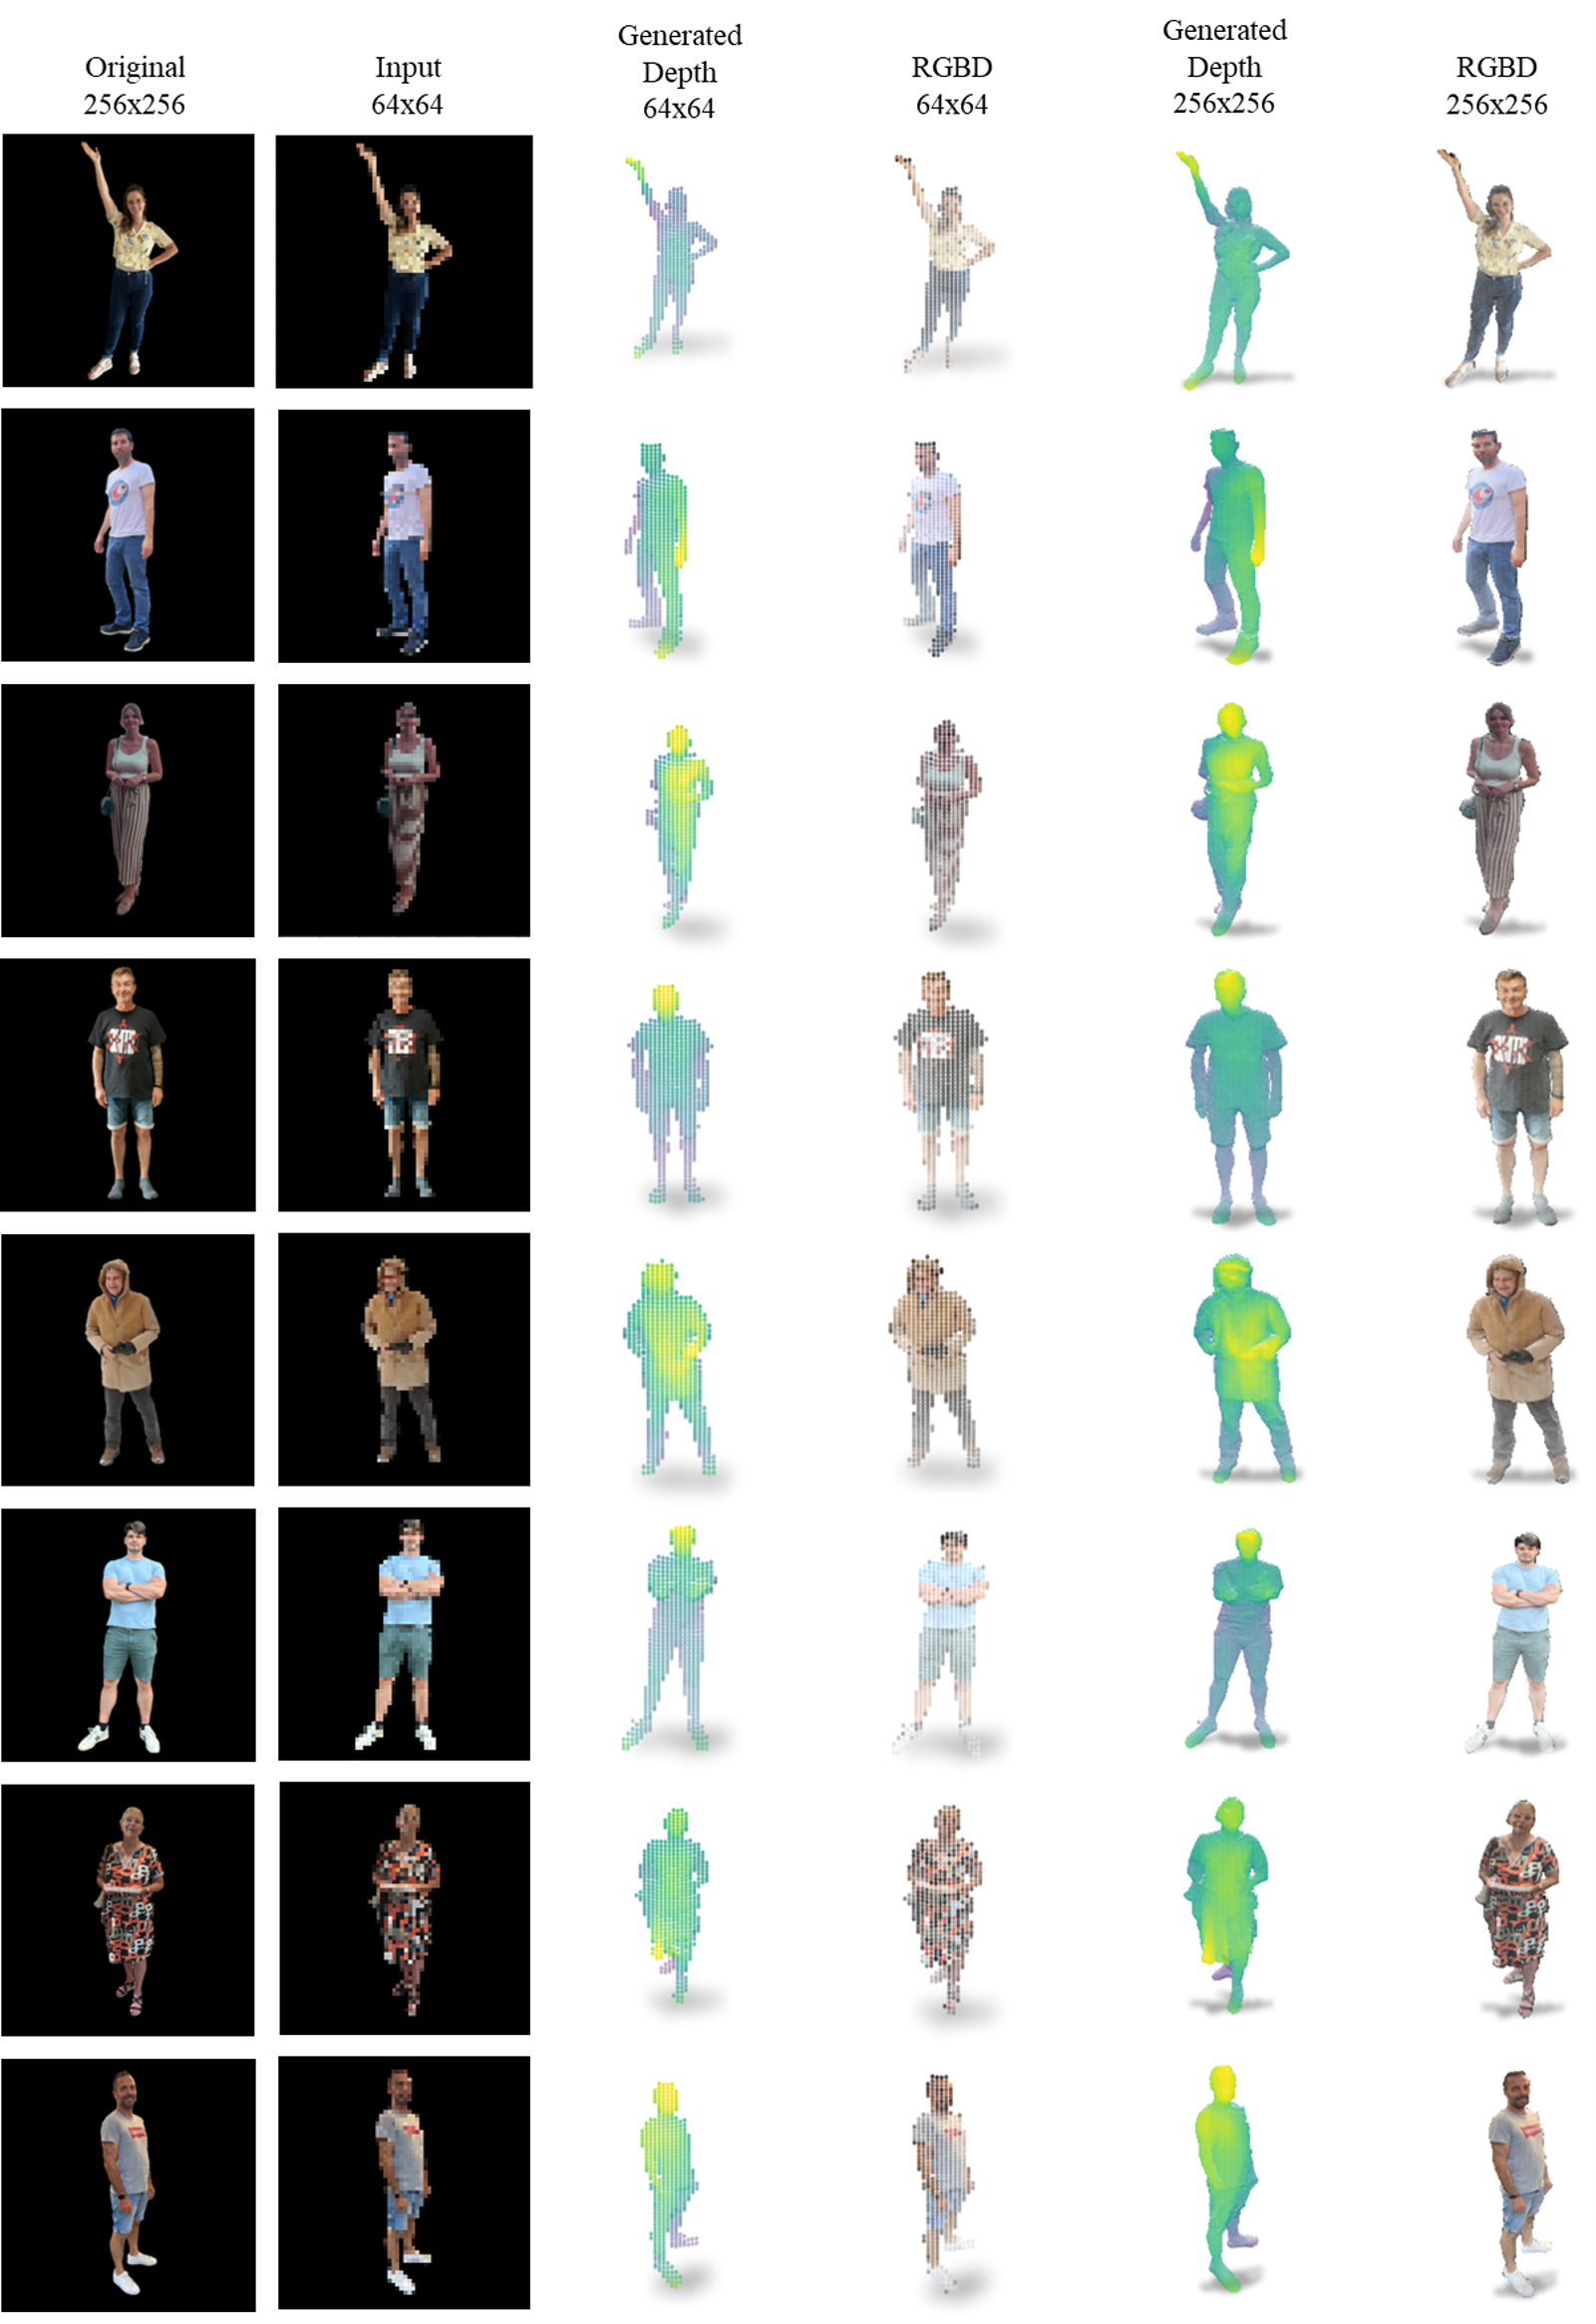
\includegraphics[width=0.95\textwidth]{illustrations/appendix_rgbd1.png}
  \label{fig:rgb_d_fusion_wild_rgbd_1}
\end{figure*}

\begin{figure*}[t]
  \centering
  \caption{Outputs of the \modelname{} framework for the given input images. Original images are taken with a variety of single-view mobile cameras.}
  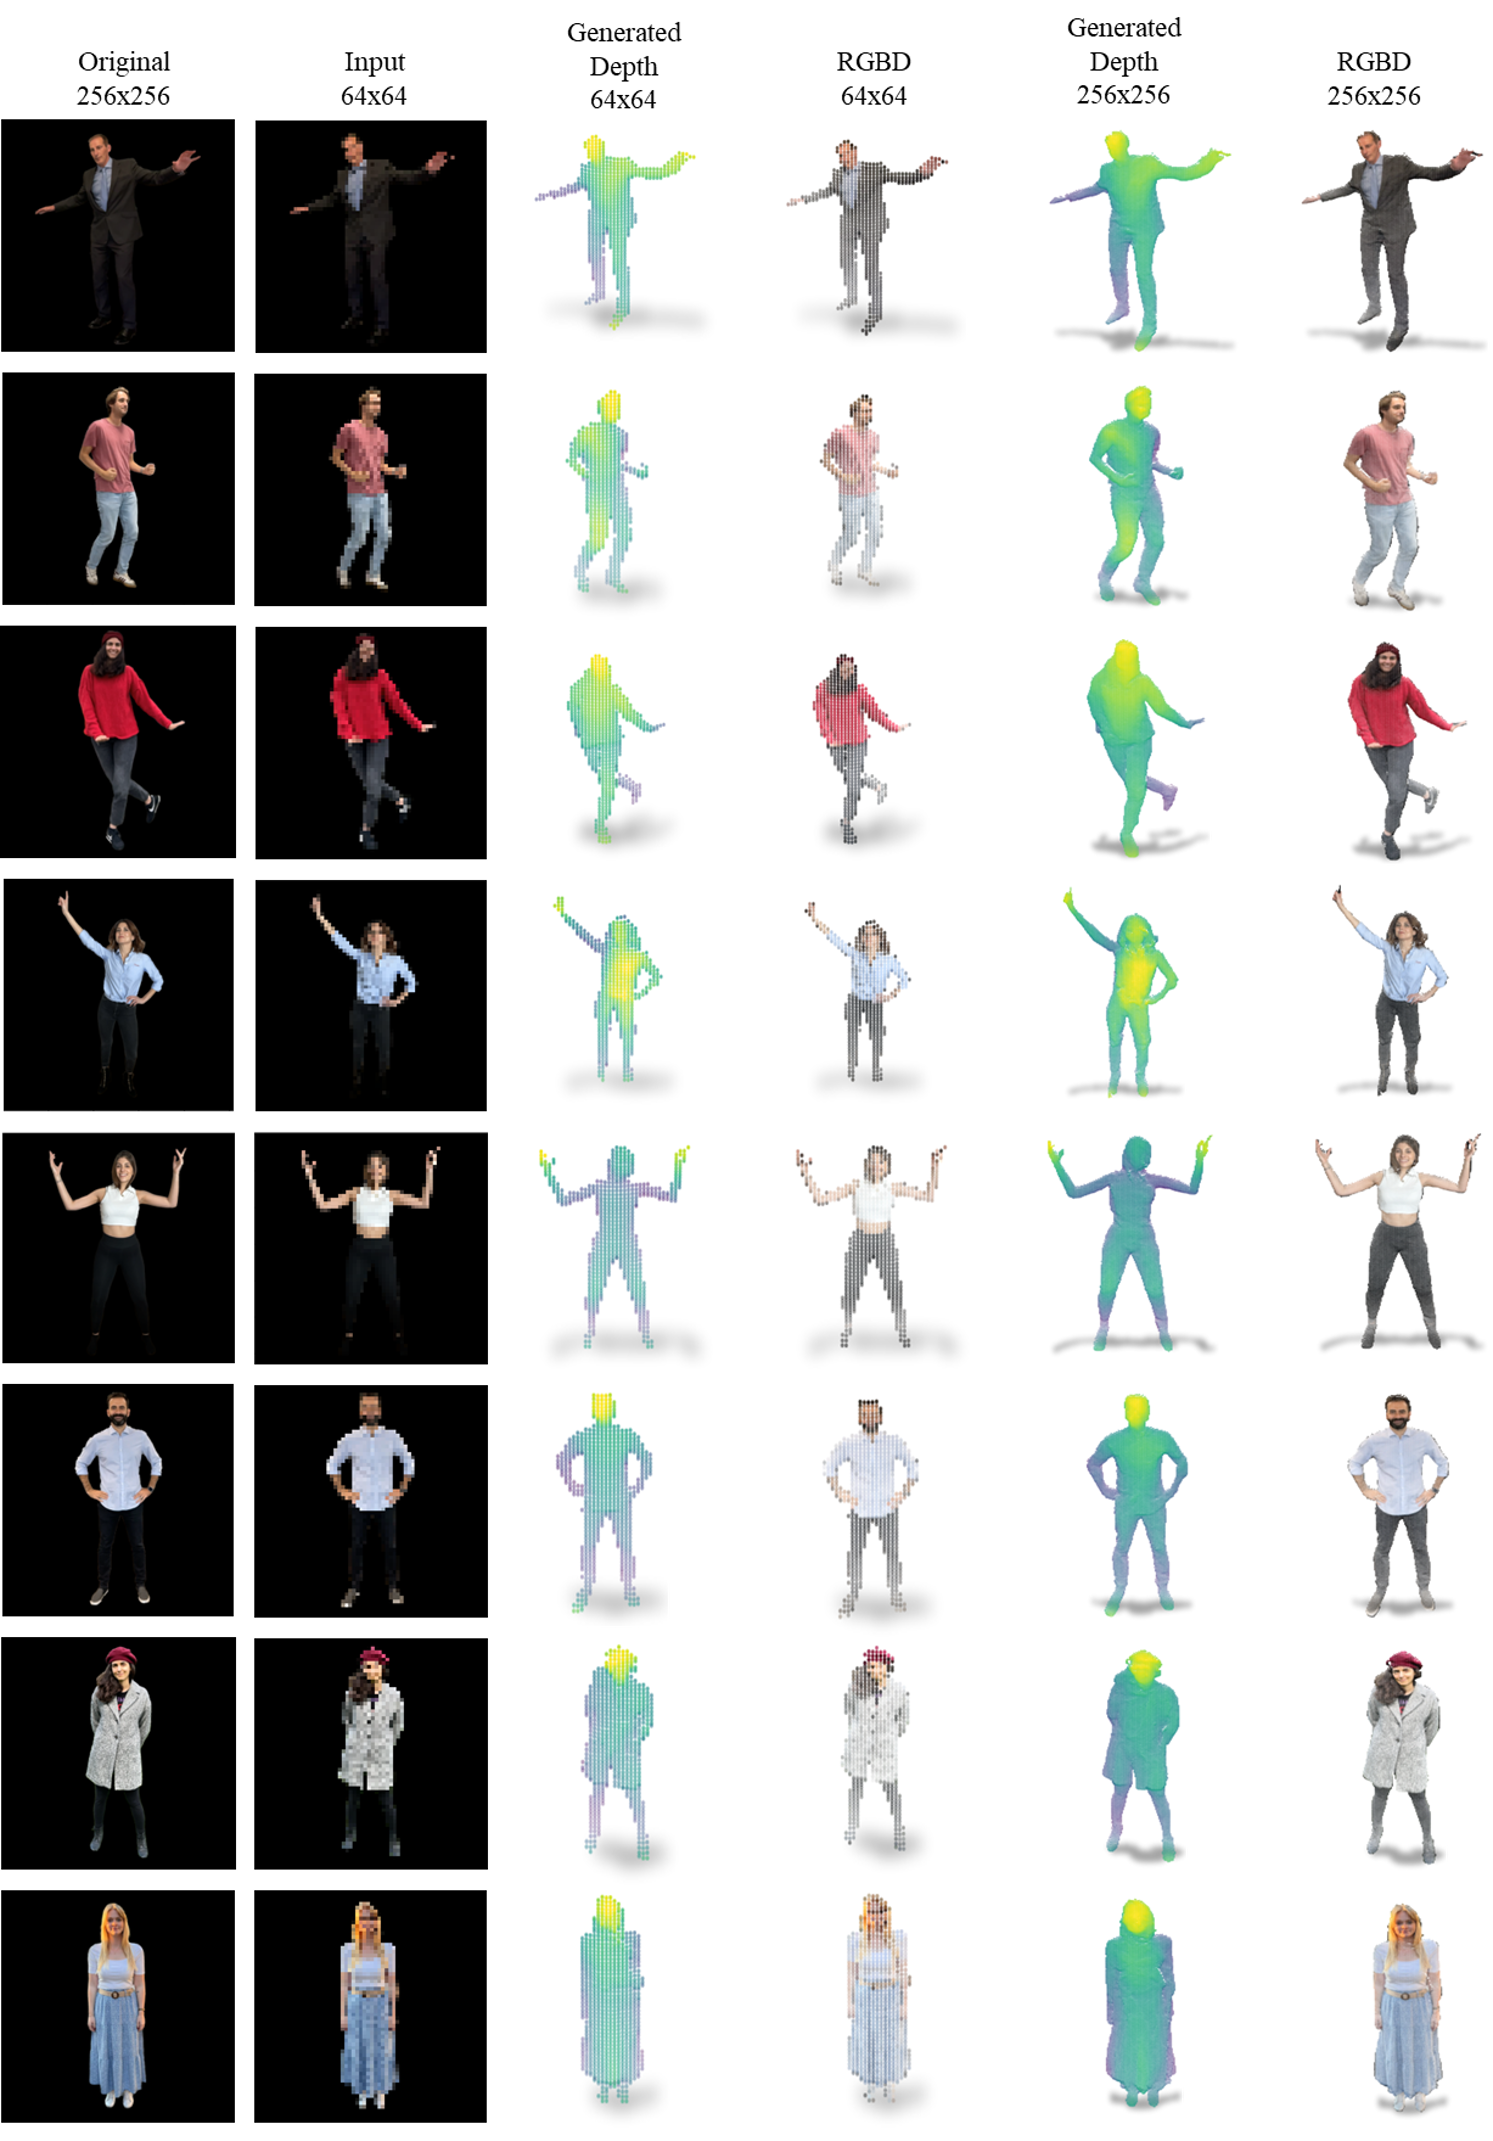
\includegraphics[width=0.95\textwidth]{illustrations/appendix_rgbd2.png}
  \label{fig:rgb_d_fusion_wild_rgbd_2}
\end{figure*}

\begin{figure*}[t]
  \centering
  \caption{Outputs of the \modelname{} framework for the given input images. Original images are generated using a stable diffusion model version 1.5 by \cite{rombach_high-resolution_2022}.}
  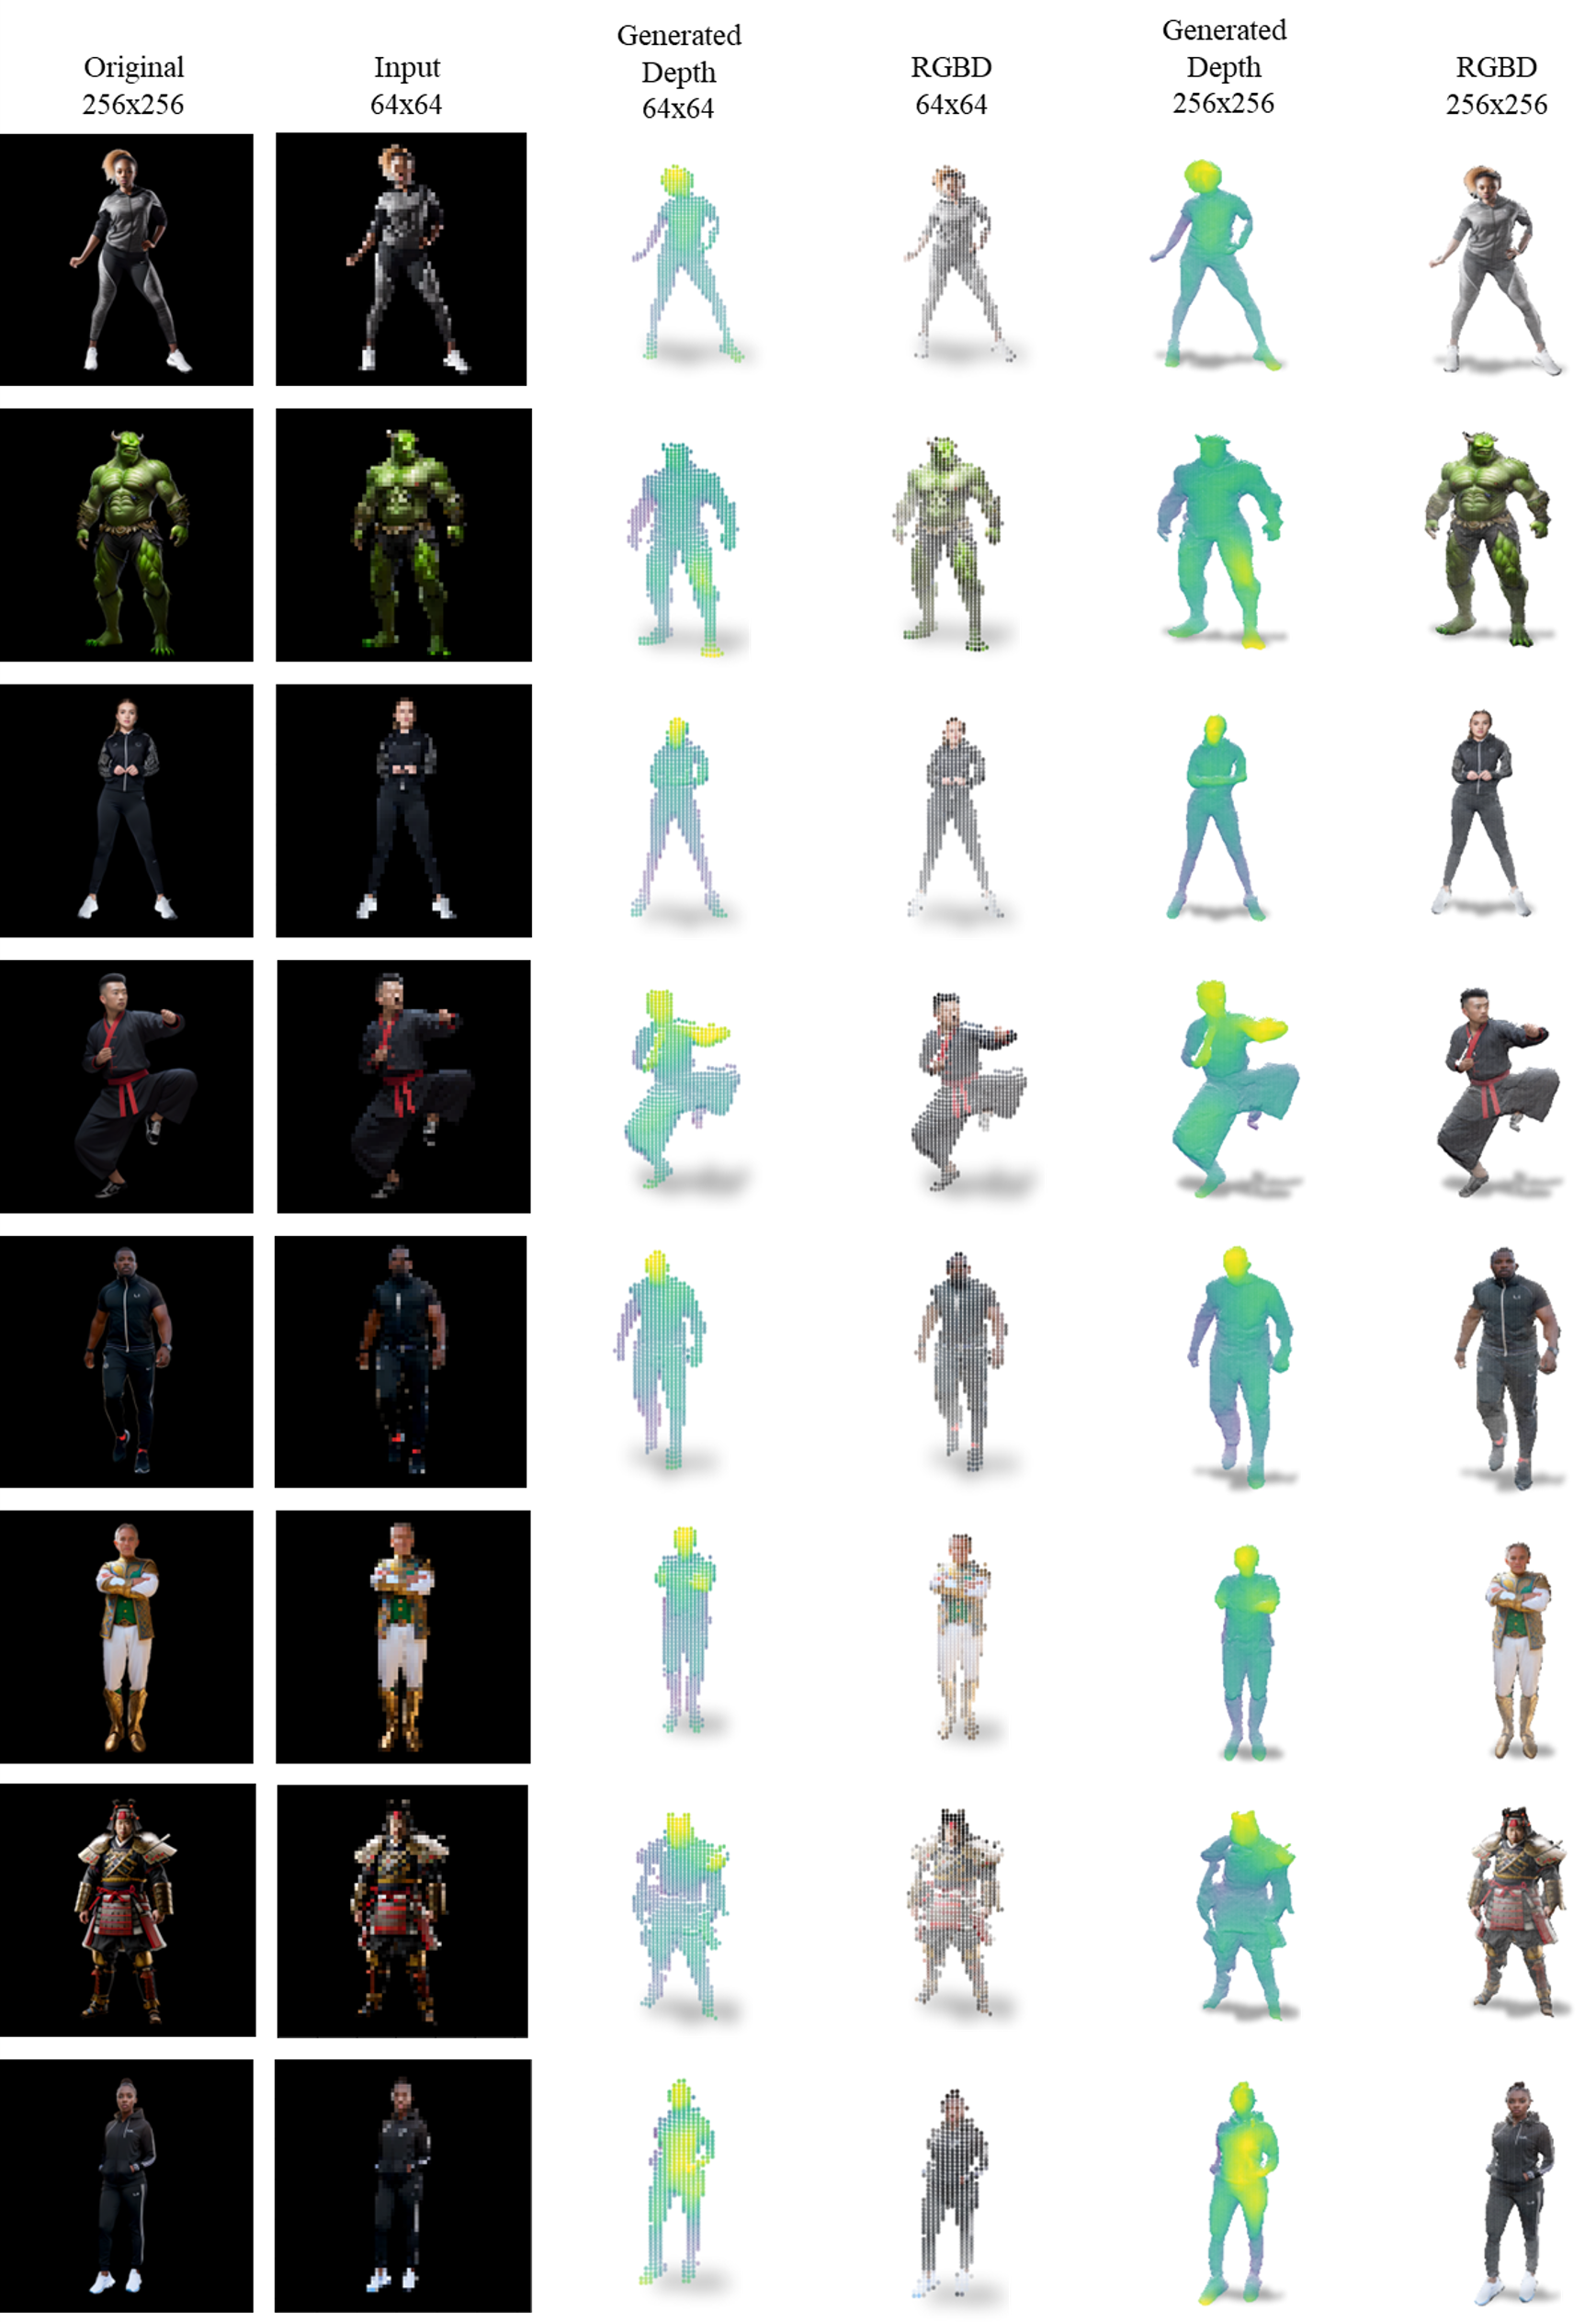
\includegraphics[width=0.95\textwidth]{illustrations/appendix_rgbd3.png}
  \label{fig:rgb_d_fusion_wild_rgbd_3}
\end{figure*}